\section{Spatio-temporal Dependence Analysis in fMRI data}

In a second application, we apply our proposed method of model selection to analyze brain activity data obtained using functional Magnetic Resonance Imaging (fMRI). Typically, the brain is divided by a grid into three-dimensional array elements called voxels, and activity is measured at each voxel. More specifically, a series of three-dimensional images are obtained by measuring Blood Oxygen Level Dependent (BOLD) signals for a time interval as the subject performs several tasks at specific time points. A single fMRI image typically consists of voxels in the order of $10^5$, which makes even fitting the simplest of statistical models computationally intensive when it is repeated for all voxels to generate inference, e.g. investigating the differential activation of brain region in response to a task.

The dataset we work with comes from a recent study involving 19 test subjects and two types of visual tasks \citep{WakemanHenson15}. Each subject went through 9 runs, in which they were showed faces or scrambled faces at specific time points. In each run 210 images were recorded in 2 second intervals, and each 3D image was of the dimension of $64 \times 64 \times 33$, which means there were 135168 voxels. Here we use the data from a single run on subject 1, and perform a voxelwise analysis to find out the effect of time lags and BOLD responses at neighboring voxels on the BOLD response at a voxel. Formally we consider two  models at voxel $i \in \{1,2,...,V\}$ at a time point $t \in \{1,2,...,T\}$.

\subsection{Temporal model} The first model we consider is a $K$-th order autoregressive model in which we try to determine the effect of time lag upto 5 past frames on the BOLD response in voxel $i$ through the coefficients $(\delta_{i1},...,\delta_{i5})$:
%
$$ y_i(t) = x_{ia}(t) \beta_{ia} + x_{ib}(t) \beta_{ib} + \sum_{l=1}^q t^{l-1} \gamma_{il} + \sum_{K=1}^5 y_i(t-k) \delta_{i,t-k} + \epsilon_i(t)
$$
%
\noindent Here $x_{ia}(t)$ and $x_{ib}(t)$ are stimulus values corresponding to the two tasks at time $t$ and $\sum_{l=1}^q t^{l-1} \gamma_{il}$ is the polynomial drift terms to account for background noise. The stimulus values are calculated through a deterministic equation given the exact time points a face (stimulus $a$) or scrambled image (stimulus $b$) is shown \citep{EloyanEtal14}.

In this analysis we consider $K=5$ and $q=2$, i.e. an AR(5) model with quadratic drift. With this specification, a very small fraction of voxels had any neighbors selected with any autoregressive effects (less than 1\%), and most of them was in empty areas, indicating noise.

\subsection{Spatial model}
Our second model is a spatial regression model which tries to determine the amount of spatial dependence that exists between neighboring voxels. For this, apart from the two stimulus term and two drift terms, we consider BOLD responses at all the immediate neighbors of a voxel as potential predictors:
%
$$ y_i(t) = x_{ia}(t) \beta_{ia} + x_{ib}(t) \beta_{ib} + \sum_{l=1}^q t^{l-1} \gamma_{il} + \sum_{n \in N_i} y_n(t) \delta_{i,n} + \epsilon_i(t)
$$
%
Here $N_i$ is the set of neighbors of voxel $i$, $\delta_{i,n}$ is the coefficient corresponding to the effect of neighbor $n$ of voxel $i$. We consider only immediate neighbors of a voxel. In 3-dimensional space there are 26 such neighbors for voxel not at the periphery of the grid, so the total number of predictors in the voxelwise model in this case is 30. We exclude any voxel on the periphery of the $64 \times 64 \times 33$ grid from the analysis. We also consider the drift term to be quadratic as before. Further, since a very small fraction of voxels were positive for lag terms in the previous temporal model, we decided not to include any autoregressive term here.

Clubbing together the stimuli, drift terms and neighbor terms into a combined design matrix $\tilde \bfX = (\tilde \bfx(1)^T,...,\tilde \bfx(T)^T)^T$ and coefficient vector $\bftheta_i$, we can write $y_i(t) = \tilde \bfx(t)^T \bftheta_i + \epsilon_i(t) $. We now estimate the set of non-zero coefficients in $\bftheta_i$ using our method. Suppose this set is $R_i$, and its subsets containing coefficient corresponding to neighbor and non-neighbor (i.e. stimuli and drift) terms are $S_i$ and $T_i$, respectively. To quantify the effect of neighbors we now calculate the corresponding $F$-statistic:
%
$$
F_i = \frac{(\sum_{n \in S_i} \tilde x_{i,n} \hat\theta_{i,n})^2}{(y_i(t) - \sum_{n \in T_i} \tilde x_{i,n} \hat\theta_{i,n})^2} \frac{|n-T_i|}{|S_i|}
$$
and obtain its $p$-value, i.e. $P(F_i \geq F_{|S_i|,|n-T_i|})$.

\ref{fig:fmrifigure} shows plots of the voxels with a significant $p$-value from the above $F$-test. Both left and right visual cortex areas show high spatial dependence, although this is much higher on the left side. Signals from the right eye are processed by the left visual cortex, and high spatial dependence among voxels in both these areas suggest that the right eye was more involved in processing visual signals for this specific subject. We also notice activity in cerebellum, the role of which in visual perception is well-documented \citep{CalhounEtal10, Kirschen10}.

In terms of future work, we aim to expand on the encouraging findings of this study and repeat the procedure on other individuals in the study. An interesting direction here might be including subject specific random effects and correlating their clinical outcomes (if any) to the observed spatial dependency patterns in their brain.

\begin{figure}
\centering
\captionsetup{font=footnotesize}
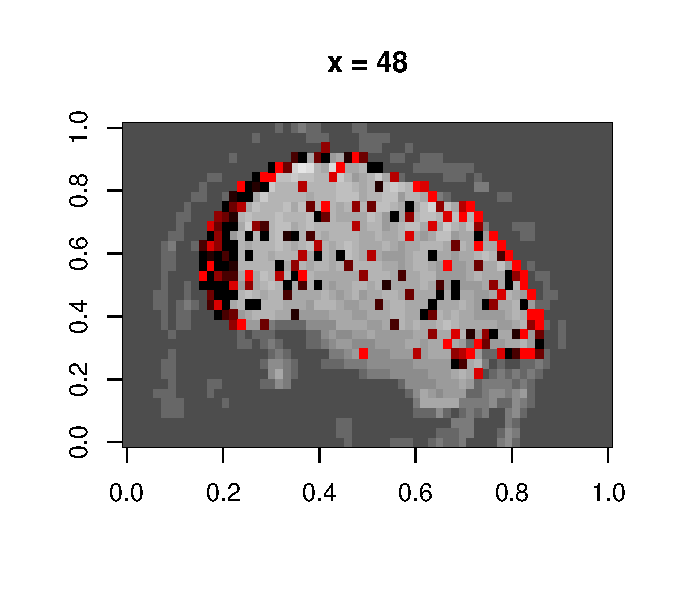
\includegraphics[width=.32\textwidth]{Chapter-appli/xslice}
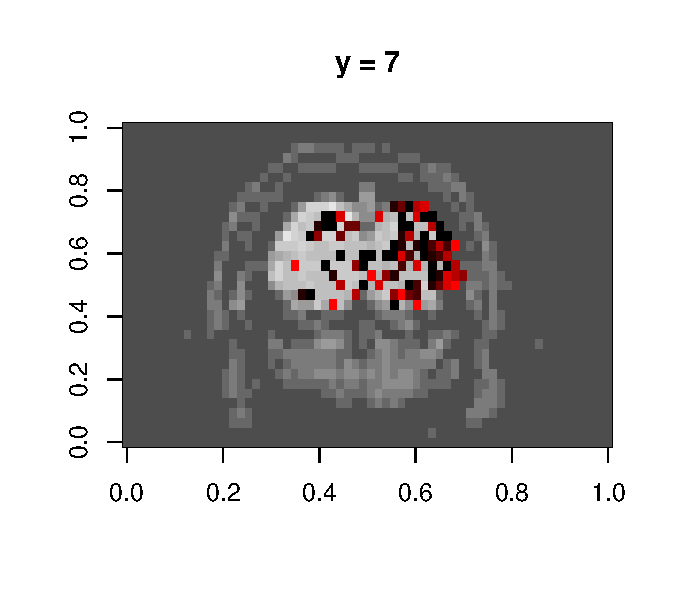
\includegraphics[width=.32\textwidth]{Chapter-appli/yslice}\\
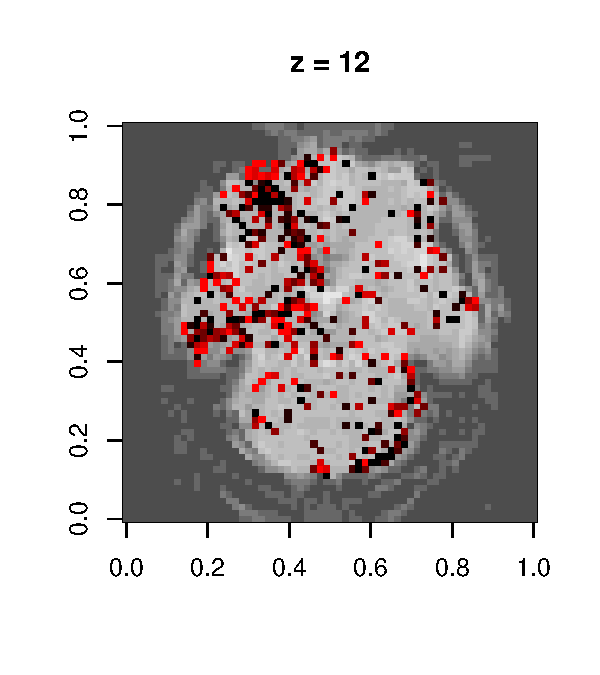
\includegraphics[width=.32\textwidth]{Chapter-appli/zslice}
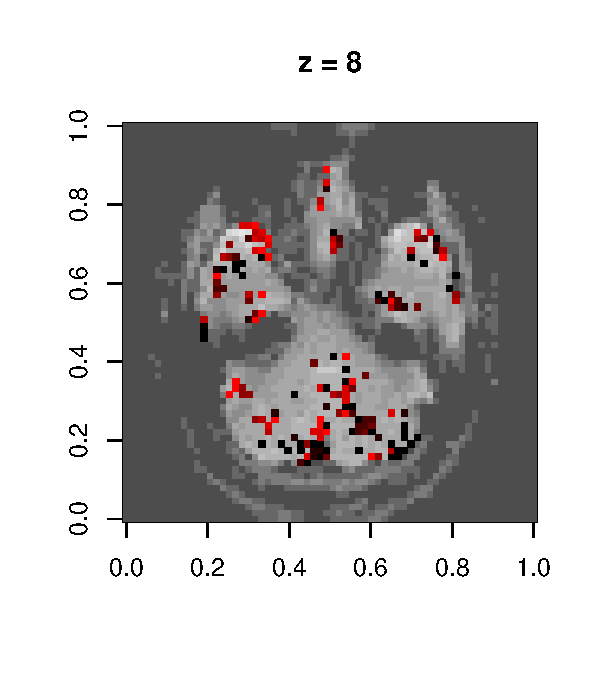
\includegraphics[width=.32\textwidth]{Chapter-appli/zslice2}\\
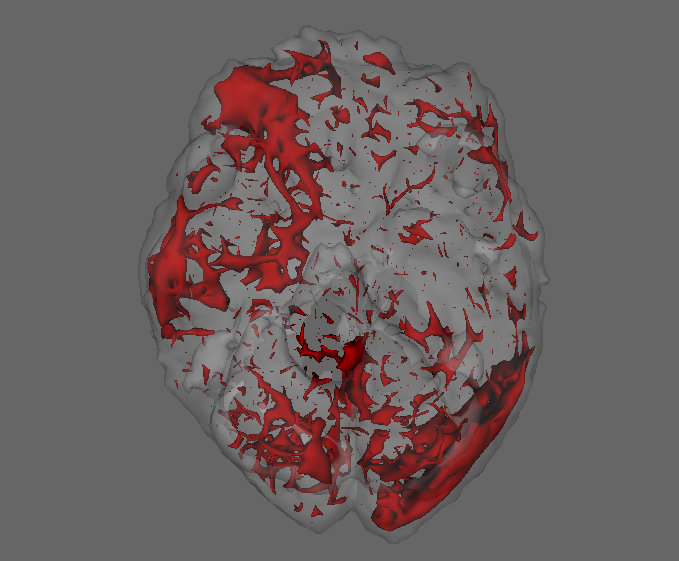
\includegraphics[width=.5\textwidth]{Chapter-appli/screenshot}

\caption{(Top) Plot of significant $p$-values at 95\% confidence level at the specified cross-sections; (bottom) a smoothed surface obtained from the $p$-values clearly shows high spatial dependence in right optic nerve, auditory nerves, auditory cortex and left visual cortex areas}
\label{fig:fmrifigure}
\end{figure}
